%% History:
% Pavel Tvrdik (26.12.2004)
%  + initial version for PhD Report
%
% Daniel Sykora (27.01.2005)
%
% Michal Valenta (3.12.2008)
% rada zmen ve formatovani (diky M. Duškovi, J. Holubovi a J. Žďárkovi)
% sjednoceni zdrojoveho kodu pro anglickou, ceskou, bakalarskou a diplomovou praci

% One-page layout: (proof-)reading on display
%%%% \documentclass[11pt,oneside,a4paper]{book}
% Two-page layout: final printing
\documentclass[11pt,twoside,a4paper]{book}   
%=-=-=-=-=-=-=-=-=-=-=-=--=%
% The user of this template may find useful to have an alternative to these 
% officially suggested packages:
\usepackage[english,czech]{babel}
\usepackage[T1]{fontenc} % pouzije EC fonty 
% pripadne pisete-li cesky, pak lze zkusit take:
% \usepackage[OT1]{fontenc} 
\usepackage[utf8]{inputenc}
%=-=-=-=-=-=-=-=-=-=-=-=--=%
% In case of problems with PDF fonts, one may try to uncomment this line:
%\usepackage{lmodern}
%=-=-=-=-=-=-=-=-=-=-=-=--=%
%=-=-=-=-=-=-=-=-=-=-=-=--=%
% Depending on your particular TeX distribution and version of conversion tools 
% (dvips/dvipdf/ps2pdf), some (advanced | desperate) users may prefer to use 
% different settings.
% Please uncomment the following style and use your CSLaTeX (cslatex/pdfcslatex) 
% to process your work. Note however, this file is in UTF-8 and a conversion to 
% your native encoding may be required. Some settings below depend on babel 
% macros and should also be modified. See \selectlanguage \iflanguage.
%\usepackage{czech}  %%%%%\usepackage[T1]{czech} %%%%[IL2] [T1] [OT1]
%=-=-=-=-=-=-=-=-=-=-=-=--=%

%%%%%%%%%%%%%%%%%%%%%%%%%%%%%%%%%%%%%%%
% Styles required in your work follow %
%%%%%%%%%%%%%%%%%%%%%%%%%%%%%%%%%%%%%%%
\usepackage{graphicx}
%\usepackage{indentfirst} %1. odstavec jako v cestine.

\usepackage{k336_thesis_macros} % specialni makra pro formatovani DP a BP
 % muzete si vytvorit i sva vlastni v souboru k336_thesis_macros.sty
 % najdete  radu jednoduchych definic, ktere zde ani nejsou pouzity
 % napriklad: 
 % \newcommand{\bfig}{\begin{figure}\begin{center}}
 % \newcommand{\efig}{\end{center}\end{figure}}
 % umoznuje pouzit prikaz \bfig namisto \begin{figure}\begin{center} atd.


%%%%%%%%%%%%%%%%%%%%%%%%%%%%%%%%%%%%%
% Zvolte jednu z moznosti 
% Choose one of the following options
%%%%%%%%%%%%%%%%%%%%%%%%%%%%%%%%%%%%%
%\newcommand\TypeOfWork{Diplomová práce} \typeout{Diplomova prace}
% \newcommand\TypeOfWork{Master's Thesis}   \typeout{Master's Thesis} 
% \newcommand\TypeOfWork{Bakalářská práce}  \typeout{Bakalarska prace}
%\newcommand\TypeOfWork{Bachelor's Project}  \typeout{Bachelor's Project}
\newcommand\TypeOfWork{Bachelor's Project}  \typeout{Bachelor's Project}

%%%%%%%%%%%%%%%%%%%%%%%%%%%%%%%%%%%%%
% Zvolte jednu z moznosti 
% Choose one of the following options
%%%%%%%%%%%%%%%%%%%%%%%%%%%%%%%%%%%%%
% nabidky jsou z: http://www.fel.cvut.cz/cz/education/bk/prehled.html

%\newcommand\StudProgram{Elektrotechnika a informatika, dobíhající, Bakalářský}
%\newcommand\StudProgram{Elektrotechnika a informatika, dobíhající, Magisterský}
% \newcommand\StudProgram{Elektrotechnika a informatika, strukturovaný, Bakalářský}
% \newcommand\StudProgram{Elektrotechnika a informatika, strukturovaný, Navazující magisterský}
%\newcommand\StudProgram{Softwarové technologie a management, Bakalářský}
% English study:
% \newcommand\StudProgram{Electrical Engineering and Information Technology}  % bachelor programe
% \newcommand\StudProgram{Electrical Engineering and Information Technology}  %master program
\newcommand\StudProgram{Software Engineering and Management}

%%%%%%%%%%%%%%%%%%%%%%%%%%%%%%%%%%%%%
% Zvolte jednu z moznosti 
% Choose one of the following options
%%%%%%%%%%%%%%%%%%%%%%%%%%%%%%%%%%%%%
% nabidky jsou z: http://www.fel.cvut.cz/cz/education/bk/prehled.html

%\newcommand\StudBranch{Výpočetní technika}   % pro program EaI bak. (dobihajici i strukt.)
%\newcommand\StudBranch{Výpočetní technika}   % pro prgoram EaI mag. (dobihajici i strukt.)
%\newcommand\StudBranch{Softwarové inženýrství}            %pro STM
%\newcommand\StudBranch{Web a multimedia}                  % pro STM
%\newcommand\StudBranch{Computer Engineering}              % bachelor programe
%\newcommand\StudBranch{Computer Science and Engineering}  % master programe
\newcommand\StudBranch{Software Engineering}

%%%%%%%%%%%%%%%%%%%%%%%%%%%%%%%%%%%%%%%%%%%%
% Vyplnte nazev prace, autora a vedouciho
% Set up Work Title, Author and Supervisor
%%%%%%%%%%%%%%%%%%%%%%%%%%%%%%%%%%%%%%%%%%%%

\newcommand\WorkTitle{Developing an accounting component for a car-sharing support information system}
\newcommand\FirstandFamilyName{Jakub Ječmínek}
\newcommand\Supervisor{Ing. Martin Komárek}


% Pouzijete-li pdflatex, tak je prijemne, kdyz bude mit vase prace
% funkcni odkazy i v pdf formatu
\usepackage[
pdftitle={\WorkTitle},
pdfauthor={\FirstandFamilyName},
bookmarks=true,
colorlinks=true,
breaklinks=true,
urlcolor=red,
citecolor=blue,
linkcolor=blue,
unicode=true,
]
{hyperref}



% Extension posted by Petr Dlouhy in order for better sources reference (\cite{} command) especially in Czech.
% April 2010
% See comment over \thebibliography command for details.

\usepackage[square, numbers]{natbib}             % sazba pouzite literatury
%\usepackage{url}
%\DeclareUrlCommand\url{\def\UrlLeft{<}\def\UrlRight{>}\urlstyle{tt}}  %rm/sf/tt
%\renewcommand{\emph}[1]{\textsl{#1}}    % melo by byt kurziva nebo sklonene,
\let\oldUrl\url
\renewcommand\url[1]{<\texttt{\oldUrl{#1}}>}




\begin{document}

%%%%%%%%%%%%%%%%%%%%%%%%%%%%%%%%%%%%%
% Zvolte jednu z moznosti 
% Choose one of the following options
%%%%%%%%%%%%%%%%%%%%%%%%%%%%%%%%%%%%%
%\selectlanguage{czech}
\selectlanguage{english} 

% prikaz \typeout vypise vyse uvedena nastaveni v prikazovem okne
% pro pohodlne ladeni prace



	 \typeout{************************************************}
	 \typeout{Language: english}
	 \typeout{Type of Work: \TypeOfWork}
	 \typeout{Study Program: \StudProgram}
	 \typeout{Study Branch: \StudBranch}
	 \typeout{Author: \FirstandFamilyName}
	 \typeout{Title: \WorkTitle}
	 \typeout{Supervisor: \Supervisor}
	 \typeout{***************************************************}
	 \newcommand\Department{Department of Computer Science and Engineering}
	 \newcommand\Faculty{Faculty of Electrical Engineering}
	 \newcommand\University{Czech Technical University in Prague}
	 \newcommand\labelSupervisor{Supervisor}
	 \newcommand\labelStudProgram{Study Programme} 
	 \newcommand\labelStudBranch{Field of Study}




%%%%%%%%%%%%%%%%%%%%%%%%%%    Poznamky ke kompletaci prace
% Nasledujici pasaz uzavrenou v {} ve sve praci samozrejme 
% zakomentujte nebo odstrante. 
% Ve vysledne svazane praci bude nahrazena skutecnym 
% oficialnim zadanim vasi prace.
% {
% \pagenumbering{roman} \cleardoublepage \thispagestyle{empty}
% \chapter*{Na tomto místě bude oficiální zadání vaší práce}
% \begin{itemize}
% \item Toto zadání je podepsané děkanem a vedoucím katedry,
% \item musíte si ho vyzvednout na studiijním oddělení Katedry počítačů na Karlově náměstí,
% \item v jedné odevzdané práci bude originál tohoto zadání (originál zůstává po obhajobě na katedře),
% \item ve druhé bude na stejném místě neověřená kopie tohoto dokumentu (tato se vám vrátí po obhajobě).
% \end{itemize}
% \newpage
% }

%%%%%%%%%%%%%%%%%%%%%%%%%%    Titulni stranka / Title page 

\coverpagestarts

%%%%%%%%%%%%%%%%%%%%%%%%%%%    Podekovani / Acknowledgements 

\acknowledgements
\noindent
I would like to thank my parents and grandparents for support, then I'd like to thank my supervisor Ing. Marin Komárek for 
accepting my request to join Metrocar team. Also I have to mention Bc. Petr Pokorný who gave me a lot of advices and recommendations about Django/Python development.


%%%%%%%%%%%%%%%%%%%%%%%%%%%   Prohlaseni / Declaration 

%\declaration{V~Kořenovicích nad Bečvárkou dne 15.\,5.\,2008}
\declaration{In Zábřeh na Moravě on December 21, 2012}


%%%%%%%%%%%%%%%%%%%%%%%%%%%%    Abstract 
 
\abstractpage

The goal of this work is to continue in development of web application Metrocar, which will be used for operating 
carsharing company. It addresses analysis, design and implementation of application which connects system Metrocar and 
accounting system Flexibee. Information system Metrocar is developed on Python platform and framework Django.

As a part of implementation of application which connects system Metrocar and system Flexibee is developed library Flexipy in Python.
This library is using REST API which is a part of system Flexibee.   
% Prace v cestine musi krome abstraktu v anglictine obsahovat i
% abstrakt v cestine.
\vglue60mm

\noindent{\Huge \textbf{Abstrakt}}
\vskip 2.75\baselineskip

\noindent
Cílem práce je pokračovat ve vývoji webové aplikace Metrocar, která bude sloužit k provozování carsharingové společnosti. Zabývá se 
analýzou, návrhem a implementací aplikace, která propojuje systém Metrocar s účetním systémem Flexibee. Informační systém Metrocar 
je vyvíjen na platformě Python za použití frameworku Django. 

V rámci implementace aplikace pro komunikaci mezi systémem Metrocar a 
systémem Felxibee je vyvíjena i knihovna Flexipy pro komunikaci se systémem Flexibee v jazyce Python. Tato knihovna využívá 
REST API, které je součástí systému Flexibee. 

%%%%%%%%%%%%%%%%%%%%%%%%%%%%%%%%  Obsah / Table of Contents 

\tableofcontents


%%%%%%%%%%%%%%%%%%%%%%%%%%%%%%%  Seznam obrazku / List of Figures 

\listoffigures


%%%%%%%%%%%%%%%%%%%%%%%%%%%%%%%  Seznam tabulek / List of Tables

\listoftables


%**************************************************************

\mainbodystarts
% horizontalní mezera mezi dvema odstavci
%\parskip=5pt
%11.12.2008 parskip + tolerance
\normalfont
\parskip=0.2\baselineskip plus 0.2\baselineskip minus 0.1\baselineskip

% Odsazeni prvniho radku odstavce resi class book (neaplikuje se na prvni 
% odstavce kapitol, sekci, podsekci atd.) Viz usepackage{indentfirst}.
% Chcete-li selektivne zamezit odsazeni 1. radku nektereho odstavce,
% pouzijte prikaz \noindent.

%**************************************************************

% Pro snadnejsi praci s vetsimi texty je rozumne tyto rozdelit
% do samostatnych souboru nejlepe dle kapitol a tyto potom vkladat
% pomoci prikazu \include{jmeno_souboru.tex} nebo \include{jmeno_souboru}.
% Napr.:
% \include{1_uvod}
% \include{2_teorie}
% atd...

%*****************************************************************************
\chapter{Introduction} \section{Carsharing definition} Carsharing is model of
renting cars where group of people is sharing car  for a short periods of
time. This is especially  usefull for people who use car only occasinally. The
organization that provides carsharing service don't have to be necessarily
comercial company, it can be cooperative, public agency or ad hoc grouping\cite{wiki:carsharing}. 

Carsharing model of renting cars is today common in North and Western Europe. In Czech Republic 
there is one company that provides this kind of services for city Brno\cite{brno}. Therefore there is still markateplace 
for another company that would provide carsharing services. 
\section{History of the project}
Project Metrocar is under development sicne year 2008. Original implementation of the project was part 
of a bachelor thesis by Bc. Ondřej Nebeský. His solution was implemented in PHP and CMS Drupal. This implementation 
allowed users to view cars on the map, create reservation for car and monitor their journeys. It also provided mechanisms 
for creating and managing carsharing subsidiaries\cite{Nebes09}. 

The final result didn't met all the requirements and also chosen architecture
wasn't optimal for the planned deployment of  the system. These shortcomings
where addressed in the master's thesis of Ing. Filip Vařecha. His goal was to
improve and transform this system.  The main goal was to create public API fot
the system. As the result, the whole system was rewritten  from scratch.
Python and Django web framework were used as primary technoliges for the
resulting system. The complete list  of changes and new features cna be found
in the thesis of Filip Vařecha\cite{Varech10}. 

Next development on the project was done as part of bachelor thesis by Bc. Jan Wágner. His main goal was to 
finish system for reservations and user managment. He was also responsible for selecting hosting for the application. 
Further details about his work on the project can be found in the resulting thesis\cite{WagneJan}. There were also some 
small contributions to the project by students of the subject Y36SI2. The complete list of their work and changes can be found 
website of the project in the final reports\cite{assembla}. 

Last contributor to the project was Bc. Petr Pokorný. He was primarly focused on the comunication between the server side of the application and car units. He was also responsible for extreme improvment in documentation of the project and updating 
project's dependecies. Thansk to his vast knowledge of Python and Django he has become importent figure of the project 
and excelent advisor. 

%*****************************************************************************
\chapter{Problem description, goal specification}
\section{Problem description}
When I joined the Metrocar project, there was only partial solution for accounting in the system. The solution was capable only to create invoices and invoice items. For printing to PDF files and sending invoices to users, there was small Python script that was supposed be running periodicly by cron and check if some invoices are supposed to be sent to the users. Also there was no way for users to gain creidt, which is basicaly curency in our system. There was alo no solution for checking 
state of company's account. Therefore the state(active, overdue and paid) of every invoice would have to be changed manually by manager of the company. This would force manager to spend to much time doing just checking statuses of invoices. Also this 
aprocha would probably fail for a larger group of users. Therefore it was decided, that system for accounting in the project 
has to be improved.
\section{Goal specification}
Design and implement application that provides connection of system Metrocar[1] to accounting software Flexibee[2]. Systems Metrocar and Flexibee will use this application for communication and exchange of data. This application will use REST API, which is provided by Flexibee[3]
Official goal specification is as follows:
\begin{itemize}
\item Identify requirements for the application.
\item Create UML models of proposed application.
\item Implement the application.
\item Create unit tests, functional tests and performance tests).
\item Create documentation for the application.
\end{itemize}

Before we decided to use for our project Flexibee as an accounting system, I was doing as a par of the subject 
A7B16PRO a research about possibilities how to connect system Metrocar to hombanking solution and accounting system.
As a result of this research, it was decided that we will use Flexibee. I decided to attach the output of my research about hombanking systems and accounting systems on Czech market to this report, because it served as a foundation for a decision to 
choose Flexibee. 

\subsection{Online banking}
Originally was system Metrocar without any kind of connection to company's bank account. Therefore, manager of company would 
have to manually check incoming payments and then change the status of appropriate invoice. This is very bad solution and it 
would be very time consuming for manager. The team that was working on the project in the year 2010 started to work on the solution, that would require create python script that would manually parse the informations about payment from email or sms that woudl be sent from bank\cite{reserse2010}. As a part of my research I found only this article about there ideas for this solution, but I wasn't capable to found any source code. Therefore I suppose they didn't impement this idea. 

At first I thought that this solution would be great for system Metrocar. I also found out that owner and founder of the Roští.cz\footnote{company that is providing hosting for project Metrocar(autonapul.cz)} Adam Štrauch created Python project that provides similar solution. His module is capable to log in to online banking system of mBank company and from there download informations about incoming payments in CSV format and then parse them into Python data structures. His project is released under BSD license and is publicly available on github\cite{python-mbank}. Article about the development of this module and the reasons for its creation can be found on his personal website\cite{mbank}. This solution is not optimal for out project, because as even author has stated, if mBank change some part of their 
online banking system, the script will simply stop to work. This is also not exactly recomended aproach to obtain this kind of 
informations. Typically every bank istituion have their own system, which allowes clients to download certain informations about payments, account status etc. These systems are called hombanking systems. There are several standard formats which 
these systems usually use. The complete list can be found here\cite{hombanking}. From my experience in these days the most used ones are Gemini, MultiCash and ABO. The basic functionality of these systems is usually same, therefore I will further describe only what Gemini in version 5.0 provides, other format support this too. 
Banking operations:
\begin{itemize}
 \item Domestic payments and direct debit orders.
 \item International payments.
 \item Domestic and international payments with future value date.
 \item Urgent payments.
 \item Permanent payment orders with automatic creation of a pre-set payment calendar.
 \item Time deposits.
\end{itemize}

Security features:
\begin{itemize}
	\item Password for electronic signature.
	\item Individual user passwords and access rights.
	\item Authorization before sending payment orders to the bank.
	\item Private and public RSA key.
	\item Electronic signatures are automaticly checked by bank institution.
\end{itemize}

Gemini has other usefull features but not all of them are supported by every hombanking system. 
The most resourcefull documentation about Gemini has Raiffeisen Bank\cite{rfb} from which I learned about this format.
Therefore these other special features might be implemented only in Raiffeisen Bank homebanking system. 

Other features of Gemini:
\begin{itemize}
	\item Export/import of payment orders to/from accounting system.
	\item Template of payment orders.
	\item Automatic communication with bank.
	\item Current exchange rates Raiffeisenbank Inc. and ČNB.
\end{itemize}
There are also other featuers, for complete list visit\cite{rfb}. When I joined the Metrocar team as a part of the A7B16PRO
subject, it was not yet decided which bank company will be used for Metrocar company's bank account. Therefore it was decided 
that my next assigment will be to select suitable accounting system for system Metrocar, which will already support communication and infromation exchange with homebanking system and that this communication will be using Gemini format and other formats too if possible. 

\subsection{Accounting system}
I was responsible for selecting appropriate accounting system for our project by the superviser Ing. Martin Komárek. I created a list of requiremnets which we expected from the accounting system. 
\begin{itemize}
	\item Capability to comunicate and exchnge data with homebanking system.
	\item The accounting system should have interface(for access from other systems).
	\item The accounting system should have sufficient documentation for developers of information systems.
	\item The aforementioned documentation should be free of charge. 
\end{itemize}
After I had this specification about what kinf of we were looking for, I started to search for the system on Czech market. 
A lot of people were telling about system Pohoda\cite{pohoda}. After small research I found that system Pohoda allows 
imports and exports of data through exchange of XML files\cite{xmlPohoda}. XSD files and example XML files are publicly avaliable and free. There is also short documentation for developers, but I found it too simple. The biggest problem with system Pohoda was tha fact that for testing of my component, I would have to purchase a license for the system. Also a lot of people who are working in companies that are using system Pohoda told me that they have negative experience with the system. 

So I started to look for other systems, until I spoke with teammate Petr
Pokrný, who recommended me accounting system Flexibee\cite{flexibee}. After some research I found out that Flexibee is 
the only accounting system on Czech market that offers completely open REST API for developers with extensive documentation, examples and tutorials. They also provide publicly available cloud version of Flexibee which developers can use for testing of their applications. Other possibility of testing is to register on their website as a developer and then they will provide full version of their system for free. They also have mailing list which they use to announce new releases and changes in their system. This is perfect ecosystem for developers. The REST API supports both XML import/export or JSON. Strongest side of Flexibee is documentation for developers. 

After I familiarized myself with Flexibee adequately I presented it to the supervisor as a solution that I would recommend and that seemed to me as the most suitable to our project and our needs. Also after discussion with Petr Pokorný who already had experience with connecting information system to Flexibee, we suggested to use Flexibee in cloud insteadof deployment on our server. This was approved by our supervisor Ing. Martin Komárek and I began to analyse existing application\footnote{Application in terms of Django application https://docs.djangoproject.com/en/dev/intro/tutorial01/\#creating-models}Invoices and what would be the best approach for connection of accounting system Flexibee. 


%*****************************************************************************
\chapter{Analysis and Solution Proposal}
In this chapter I will provide analysis of my solution on how to connect existing system Metrocar to an accounting system Flexibee. I will describe reasons for chosen approach and technologies.
\section{Invoices application}
Application invoices in project Metrocar has responsibilities for CRUD operations with invoices and other accounting documents.
It also contains tools for printing invoices and sending them to users(customers). This application was originally 
created by Filip Vařecha and then maintained by Jan Wágner. As I mentioned before, this solution has many shortcomings. Therefore as a part of this project I am supposed to connect system Metrocar to system Flexibee. At first I planned to remove application Invoices and replaced it by new application that would be directly connected to Flexibee. However as it turned out 
this application is very integrated into the Metrocar system. Also the standard things like managing invoices is well hnadled by the application. Flexibee is very good system and has a lot of happpy customers, but even systems like this expoerience from time to time poblems. Petr Pokorný expereinced a few server crashes while he was working on the project that involved Flexibee as an accounting system. At that point the whole system is inaccessible for users. because they can't create invoices or issue their bills. A this point keeping and old Invoices application could help. When a user create invoice, or issue a bill or just do some action that involves accounting and at this point Flexibee crashes, accounting module(later described) will notice this and set certain actions into motion. Accounting module will use old Invoices application and store the canges or new data in local database in apropriate tables. Also he notifes manager that server on which is Flexibee deployed has crashed. After server with Flexibee is running again, accounting module will resolve incosistences between local database and Flexibee's recors. This way we can say that old Invoices application will serve as some kind of fail-safe mechanism, which will be primarly used to serve users' requests while Flexibee is down. For this reasons I've decided to keep old application Invoices in the project Metrocar. It will be slightly modified and certian functionalities will be transfered on to Flexibee(for example printing of invoices and sending them to users). 	

\section{Accounting module}
As was metioned above, the accounting module will be responsible for handling situations in which Flexibee has crashed, but this will be only secondary purpose of this module. The main purpose of this module will be to act as intermidiate between Metrocar system and Flexibee. It will define interface for Metrocar system through which will system Metrocar interact with Flexibee. Thanks the nature of Python, this module can be easily replaced in the future with diffrent implementation of the same interface, so on the side of Metrocar system, it will look like that nothing has changed, but actually Metrocar system will now comunicate with completely diffrent accounting system on the other side. Therefore there will be no coupling between Metrocar system and Flexibee. This is very important because if the interface of accounting module was coupled with Flexibee it would extremely hard and tedious to change accounting system. 

On the side of Flexibee system, the accounting module will use library flexipy which will be described in the next section. This will also help to adhere separation of concerns pricniple\cite{wiki:soc}, because accounting module will simply call function from flexipy and passes data if needed. It will not know anything about Flexibee REST API or format of data in which Flexibee comunicate.  

\section{Flexipy}


%*****************************************************************************
\chapter{Implementation}
Popis implementace/realizace se zaměřením na nestandardní části řešení.


%*****************************************************************************
\chapter{Testing}

\begin{itemize}
 \item Způsob, průběh a výsledky testování.
 \item Srovnání s existujícími řešeními, pokud jsou známy.
\end{itemize} 


%*****************************************************************************
\chapter{Summary}

\begin{itemize}
\item Zhodnocení splnění cílů DP/BP a  vlastního přínosu práce (při formulaci je třeba vzít v potaz zadání práce).
\item Diskuse dalšího možného pokračování práce.
\end{itemize} 

%*****************************************************************************
% Seznam literatury je v samostatnem souboru reference.bib. Ten
% upravte dle vlastnich potreb, potom zpracujte (a do textu
% zapracujte) pomoci prikazu bibtex a nasledne pdflatex (nebo
% latex). Druhy z nich alespon 2x, aby se poresily odkazy.

% originally following specification for bibliography formating was used
%\bibliographystyle{abbrv}

% Here is an improvment by Petr Dlouhy (April 2010).
% It is mainly for supervisors who expect Czech fomrating rules for references
% Additional feature is live url addresses to sources from your pdf file
% It requires the file csplainnat.bst (included in this sample zipfile).

\bibliographystyle{csplainnat}

%bibliographystyle{plain}
%\bibliographystyle{psc}
{
%JZ: 11.12.2008 Kdo chce mit v techto ukazkovych odkazech take odkaz na CSTeX:
\def\CS{$\cal C\kern-0.1667em\lower.5ex\hbox{$\cal S$}\kern-0.075em $}
\bibliography{reference}
}

% M. Dušek radi:
%\bibliographystyle{alpha}
% kdy citace ma tvar [AutorRok] (napriklad [Cook97]). Sice to asi neni  podle ceske normy (BTW BibTeX stejne neodpovida ceske norme), ale je to nejprehlednejsi.
% 3.5.2009 JZ polemizuje: BibTeX neobvinujte, napiste a poskytnete nam styl (.bst) splnujici citacni normu CSN/ISO.

%*****************************************************************************
%*****************************************************************************
\appendix



% JZ: 3.5.2009 \chapter z book zajistí automaticky
%\subsection{Začátky kapitol na liché stránky}
%Ve výsledném textu je dobré, když každá kapitola začíná na liché stránce. Tedy použijte:
%\begin{verbatim}
%  \cleardoublepage\include{1_uvod}
%  \cleardoublepage\include{2_teorie}
%   atd.\ldots{}
%\end{verbatim}

%*****************************************************************************
\chapter{Seznam použitých zkratek}

\begin{description}
\item[XML] Extensible Markup Language
\item[JSON] JavaScript Object Notation
\item[API] Application programming interface
\item[REST] Representational state transfer
\item[CSV] Comma-separated values
\end{description}
\vdots

%*****************************************************************************
\chapter{UML diagramy}
\textbf{\large Tato příloha není povinná a zřejmě se neobjeví v každé práci. Máte-li ale větší množství podobných diagramů popisujících systém, není nutné všechny umísťovat do hlavního textu, zvláště pokud by to snižovalo jeho čitelnost.}

%*****************************************************************************
\begin{figure}[h]
\begin{center}
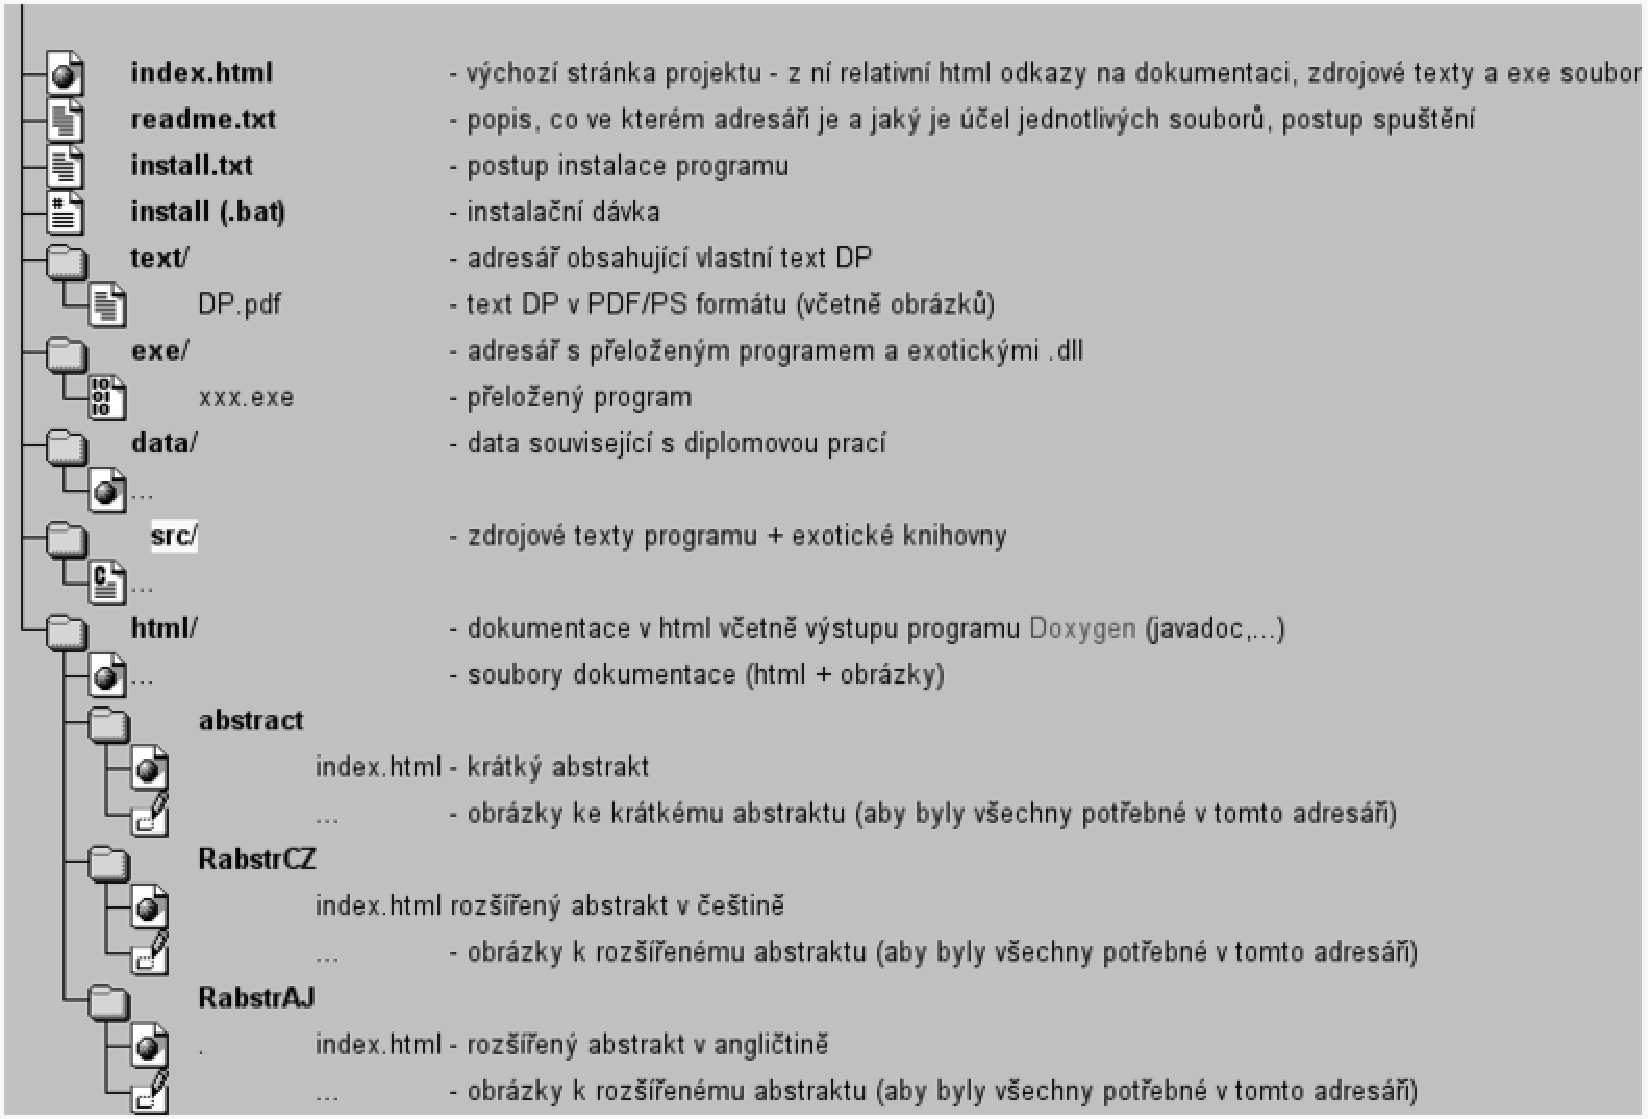
\includegraphics[width=14cm]{figures/seznamcd}
\caption{Seznam přiloženého CD --- příklad}
\label{fig:seznamcd}
\end{center}
\end{figure}

\end{document}
